\documentclass{article}

\usepackage{microtype}
\usepackage{graphicx}
\usepackage{subfigure}
\usepackage{booktabs}

\usepackage{hyperref}
\newcommand{\theHalgorithm}{\arabic{algorithm}}

\usepackage{icml2023}
% \usepackage[accepted]{icml2023}  % uncomment for camera ready

\icmltitlerunning{Maximum Likelihood Estimation for Molecular Counts}

\begin{document}

\twocolumn[
  %\icmltitle{A Differentiable Markov-Chain for Maximum Likelihood Estimation of Molecular Counts}
  \icmltitle{A Differentiable Markov-Chain to Estimate\\ the Number of Fluorescent Emitters from Intensity Traces}

  \begin{icmlauthorlist}
  \icmlauthor{Alexander Hillsley}{janelia}
  \icmlauthor{Johannes Stein}{wyss}
  \icmlauthor{Paul Tillberg}{janelia}
  \icmlauthor{David Stern}{janelia}
  \icmlauthor{Jan Funke}{janelia}
  \end{icmlauthorlist}

  \icmlaffiliation{janelia}{HHMI Janelia Research Campus, Ashburn, VA}
  \icmlaffiliation{wyss}{Wyss Institute for Biologically Inspired Engineering, Harvard University, Boston, MA}
  \icmlcorrespondingauthor{Alexander Hillsley}{hillsleya@janelia.hhmi.org}

  \icmlkeywords{Machine Learning, ICML, Differentiable Model, Markov-chain, Fluorescence Microscopy, Molecular Counting}

  \vskip 0.3in
]

\begin{abstract}

  We address the problem of inferring the number of independently blinking
  \introduce{fluorescent light emitters}, when only the sum of all of their
  \introduce{intensity} contributions can be observed at each
  \introduce{timepoint}.
  %
  % why do we want to do that?
  %
  This problem occurs regularly in light microscopy of \introduce{complexes}
  that are smaller than the diffraction limit, where one wishes to count the
  number of \introduce{fluorescently} labelled \introduce{subunits}.
  %
  % how do we do that?
  %   differentiable markov chain
  %   blinx estimates number of active emitters for each timestep
  %   holistic model
  %
  We estimate the number of subunits of a complex by modelling the light
  emitted per complex over time as a Markov-chain.
  %
  Crucially, our model is differentiable, which allows us to jointly estimate
  the parameters of the intensity distribution per emitter as well as their
  blinking rates through maximum likelihood optimization.
  %
  % how good is it?
  %
  Compared to the current state of the art, which uses histogram-based
  heuristics to infer distribution parameters, our holistic model is
  consistently more accurate and extends the range of countable subunits by a
  factor of two.
  %
  Furthermore, our model allows us to inform experimentalists about optimal
  imaging parameters to increase accuracy.

\end{abstract}

\section{Introduction}

% counting structures is important
% super resolution to the rescue
%
Fluorescence microscopy is a foundational tool in the field of biology and
provides useful information on the abundance and localization of labeled
structures.
%
  However, determining the exact molecular count of subunits in a complex
  remains a challenge. Super-resolution techniques such as PALM
  \cite{betzig_imaging_2006}, STORM \cite{rust_sub-diffraction-limit_2006}, and
  DNA-PAINT \cite{schnitzbauer_super-resolution_2017} have addressed this
  problem by achieving resolutions as high as 20nm.

% key concept of super-resolution: fluorescence over time
% doesn't work for many very small structures
%
The underlying principle that overcomes the diffraction limit of light is the
distribution of fluorescence signals from individual fluorophores over time:
%
  only a sparse subset of fluorescent emitters are \introduce{\emph{active}}
  (\ie, emitting light) at each point in time.
  %
  Each spatially distinct emitter can then be localized with sub-pixel accuracy
  by fitting its point spread function. Subsequently, all localizations over
  all frames can be combined into a sub-diffraction limited reconstruction.
  %
  Although the subunits of some complexes can be sufficiently spatially
  separated with super-resolution techniques for visual counting, many exist
  even below this threshold, prompting the need for new methods of molecular
  counting.

% intro to molecular counting for computer scientists: what is the data, what
% do we want to predict?
%
The challenge for molecular counting is then to disentangle the contributions
of multiple fluorescent emitters that overlap in space.
%
  % multiple emitters, single spot
  % intensity trace of combined intensity
  % unknown number of active emitters per timepoint
  % noisy measurements, randomly distributed with unknown parameters
  % dependency on "kinetics" of emitters
  %
  % -> joint inference problem: number of active emitters per timepoint and
  %    parameters
  This problem is ill-posed in a static image, where the intensities of all
  emitters are combined into a single \introduce{spot}. However, the
  fluctuating \introduce{intensity trace} over time can provide enough
  information to infer the number of emitters:
  %
  %While this problem is ill-posed in a static image, the fluctuating
  %\introduce{intensity trace} of the combined intensity of independently
  %blinking emitters over time in a single \introduce{spot} can provide enough
  %information to infer the number of emitters:
  %
  At each timepoint, a subset of all emitters will be active, and thus
  contribute to the combined intensity. Between timepoints, the number of
  active emitters changes accordingly to their underlying \introduce{blinking
  rates}.
  %
  None of the parameters of this process (\eg, intensity of a single emitter,
  probability of activating or deactivating) are known \emph{a-priori} and need
  to be inferred jointly with the total number of emitters.

Here we propose \ours, a differentiable Markov-chain model for intensity
traces, which is conditioned on the total number of emitters, the parameters of
the intensity distribution, and the blinking rates.
%
  \ours allows joint estimation of the parameters of the intensity distribution
  per emitter as well as their blinking rates through maximum likelihood
  optimization.
  %
  The most likely number of emitters per trace is then found as the maximum
  \emph{a-posteriori} solution.

We compare \ours on synthetic traces (where the true number of emitters is
known) and compare its predictions against the current state-of-the-art method,
\lbfcs~\citep{stein_calibration-free_2021}.
%
  \ours is consistently more accurate than \lbfcs and extends the range of
  countable subunits by a factor of two.
  %
  Furthermore, we show that \ours can be used to inform experimental design by
  identifying conditions that facilitate molecular counting.

\paragraph{Related Work}

% molecular counting
Many molecular counting approaches similarly
  make use of imaging over time to extract additional information from the
  system. Some of the simplest systems count events that are designed to happen
  only once per label such as photobleaching steps \cite{Ulbrich_subunit_2007} or
  blinks from a 1 time photo-switching fluorophore
  \cite{gunzenhauser_quantitative_2012}. However, these events are often difficult to
  detect, and can easily be missed leading to severe undercounting.

Other methods make use of fluorophores that blink repeatedly to reduce the
dependence on individual events.
%
  By modeling the photoswitching kinetics of STORM dyes as a continuous time
  Markov process, \cite{patel_blinking_2021, rollins_stochastic_2015} one can extract the total count of molecules
  in a given area. However, these models are limited in accuracy by the complex
  photobleaching nature of the dyes used. Another temporal counting method is
  qPAINT \cite{jungmann_quantitative_2016} which utilizes DNA-PAINT to minimize photobleaching and
  correlates the frequency of repeated binding and unbinding events to the
  molecular count. This method shows an excellent accuracy for counts under 15,
  but relies heavily on previous knowledge of binding kinetics and is
  susceptible to simultaneous binding events.

Although not precise enough to determine molecular counts, the linear
relationship observed between fluorescence intensity and fluorophore abundance
\cite{schmied_fluorescence_2012}, provides additional information to improve the
accuracy of these methods.
%
  Many methods use correlation functions to combine both the temporal and
  intensity information to estimate the molecular count, such as balanced
  super-resolution optical fluctuation imaging (bSOFI) and fluorescence
  correlation spectroscopy (FCS) which has been used to estimate the copy
  number of specific proteins within the nuclear pore complex
  \cite{otsuka_quantitative_2023}. Similar techniques have also been applied to the
  consistent blinking behavior of DNA-PAINT in lbFCS+ \cite{stein_calibration-free_2021}, which has
  accurately counted up to ~8 molecules and does not rely on previous
  calibrations. These models work by fitting the entire observation series to a
  single equation, in the process greatly simplifying the information. We
  hypothesize that by fitting the entire observation series our model will be
  able to use this additional information to greatly improve the counting
  accuracy of our model.

\todo{merge somewhere above?}
A further advantage of \ours is that it produces a likelihood distribution
across all possible counts, that could be useful for further downstream
applications.


\section{Method}

Consider a complex of fluorescent emitters, smaller than can be visually separated. Each emitter activates stochastically and independently of the others, producing a signal of fluctuating intensity over time \figref{fig:results:comparison}.
The goal of this method is to determine the true number of emitters \truen given the observed intensity trace.

\subsection{Model}

First, focusing on only a single timepoint $t$, we need an emission distribution to describe the relationship between the number of active emitters \y{t} and the observed intensity \x{t}. The individual intensities of multiple emitters are additive, and can be approximated by a log-normal distribution \cite{mutch_deconvolving_2007} \ie.
%
\begin{equation*}
  p(\x{t}|\y{t}, \mu, \sigma) =
    \frac{1}{\x{t}\sigma\sqrt{2\pi}}
    \exp \left(
      - \frac{|\log(\x{t}) - \y{t}\mu|^2}{2\sigma^2}
    \right)
  \text{,}
\end{equation*}

Where $\mu$ and $\sigma$ are the mean and standard deviation of the intensity of a single active emitter.

Next, to model the temporal fluctuations in intensity, observed in the trace \trace, we need a distribution to describe the change in the number of active emitters \states over time. To do this, we assume that the process is Markovian and the number of active emitters \y{t} at time $t$ is only dependent on the number of active emitters at the previous timepoint \y{t-1}. Breaking down the system to each individual emitter, we define the probability that an emitter that is active at time $t-1$ becoming inactive at time $t$ as \poff, conversely, we define the probability that an emitter inactive at time $t-1$ becoming active at time $t$ as \pon. Finally, assuming that all emitters share the same \poff and \pon, the transition distribution can be written as:
%
\begin{align*}
  p(\y{t} = y | \y{t-1}, \n, \pon, \poff) &=\\
	\sum_{a = 0}^{\y{t-1}}
    {a \choose \y{t-1}}
    &\pon
    {y - \y{t-1} + a \choose \n - \y{t-1}}
    \poff
\end{align*}
%
Where $a$ is the number of emitters changing state. Note that this distribution depends on the total number of available emitters
\n, as the probability of a change in the number of activate transmitters
depends on the total number of emitters available.

Expanding these distributions to account for entire intensity trace \trace and marginalizing over all possible \states, we can build a distribution for the probability of observing trace \trace given total number of emitters \n and simplifying the emission and transition distributions with $\parameters = (\pon, \poff, \mu, \sigma)$

\begin{align*}
  p(\trace|\n,\parameters) &=\\
    \sum_{\states}
      p(&\x{1}|\y{1}, \parameters)
      p(\y{1}|\n, \parameters)
      \prod_{t=2}^{T}
        p(\x{t}|\y{t}, \parameters)
        p(\y{t}|\y{t-1},\n, \parameters)
  \label{eq:method:likelihood}
\end{align*}

Maximum likelihood estimation can then be used to find the \parameters that best fit the observation \trace, given \n. 
Finally this process can be repeated for all possible values of n, and maximum likelihood estimation used to find the estimated number of emitters in the system \estimatedn:

\begin{equation}
    \estimatedn =
    \argmax{\n}
    \max_\parameters
    p(\trace|\n,\parameters)
  \text{.}
  \label{eq:method:optimization}
\end{equation}

\subsection{Inference}

Because there is no closed form solution to  \eqref{eq:method:optimization} we can use gradient ascent to find the optimal $\theta$ given \n.
The gradient of the likelihood function $p(\trace | \n, \theta)$ was calculated using JAX, an auto-differentiation library.
This was done recursively, as is standard for hidden Markov models, through the forward algorithm.
The likelihood $p(\trace | \n, \theta)$ was defined recursively through \pchain(\y{t}), the probability of observing the sequence of events 0 through $t$.
Therefore the probability of observing trace \trace is $ p(\trace|\n,\parameters) = \sum_{\y{T}} \pchain_T(\y{T})$ and, omitting \n and \parameters for simplicity, \pchain(\y{t})  is defined as:

\begin{align*}
  \pchain_{t}(\y{t}) &= p(\x{t}|\y{t}) \sum_{\y{t-1}} p(\y{t} | \y{t-1}) \pchain_{t-1}(\y{t-1})\\
  \pchain_{1}(\y{1}) &= p(\x{1}|\y{1}) p(\y{1})
\end{align*}

Because $\pchain_{t}$ depends multiplicatively on the previous $\pchain_{t-1}$,
the probability becomes vanishingly small for large times $t$, leading to
numerical stability problems. Further, because there is a marginalization over
\states at each $t$, the standard trick of moving to log space, is not
effective.

To alleviate this issue, we introduce a normalized recursive scheme, where
$\pchainnorm$ are normalized to sum up to one for all \y{}:
%
\begin{align*}
  \pchainnorm_t(\y{t}) &=
    \frac{1}{\norms_t}
    p(\x{t}|\y{t})
    \sum_{\y{t-1}}
      p(\y{t} | \y{t-1})
      \pchainnorm_{t-1}(\y{t-1})\\
  \pchainnorm_{1}(\y{1}) &=
    \frac{1}{\norms_1}
    p(\x{t}|\y{t})
    p(\y{t})\\
  \norms_t &=
    \sum_{\y{}}
    p(\x{t}|\y{})
    \sum_{\y{t-1}}
      p(\y{} | \y{t-1})
      \pchainnorm_{t-1}(\y{t-1})\\
  \norms_1 &=
    \sum_{\y{}}
    p(\x{1}|\y{})
    p(\y{1})  \text{.}\\
\end{align*}
%
The original $\pchain_{t}$ can now be recovered by denormalizing $\pchainnorm_{t}$:
%
\begin{equation*}
  \pchain_t(\y{t}) = \pchainnorm_t \prod_{t'=1}^t \norms_{t'}
  \text{.}
\end{equation*}
%
In fact, because the sum of $\pchain_{t}$ over all \y{t} is one by definition, the measurement likelihood is now equivalent to the product of all normalization factors:
%
\begin{align*}
  p(\trace|\n,\parameters)
    &= \sum_{\y{T}} \pchainnorm_{t}(\y{T}) \prod_{t'=1}^T \norms_{t'}\\
    &= \left( \prod_{t'=1}^T \norms_{t'} \right)
      \underbrace{\sum_{\y{T}} \pchainnorm_{t}(\y{T})}_{=1}
    = \prod_{t'=1}^T \norms_{t'} ,\text{.}\\
\end{align*}
%
This allows us to compute the measurement likelihood from a single product,
which can be done in log space to ensure numerical stability.

\section{Results}

\begin{figure*}

  \begin{panel}{(a)}{\textwidth}
    \def\histogramcsv{figures/data/sim_counting/intensity_histogram.csv}
    \def\tracecsv{figures/data/sim_counting/trace_and_fit_N10.csv}
    \def\traceintensitycol{trace}
    \def\zcol{fit}
    \def\histbincol{N10_bins}
    \def\histcountcol{N10_measured}
    \def\modelfitcol{N10_model}
    \def\posteriorcsv{figures/data/sim_counting/posteriors.csv}
    \def\posteriorcol{posterior_10}
    \hspace{-2mm}
    \tikzsetnextfilename{figure_2_trace_N10}
    \begin{tikzpicture}
      \node (fancyplot) {\begin{tikzpicture}%
  \begin{axis}[
    name=trace,
    width=0.8\textwidth,
    height=5cm,
    xlabel=frames,
    ylabel=intensity,
    enlarge x limits=false,
    xtick distance=500,
    grid=major,
    grid style={dashed},
    scaled ticks=false,
    ticklabel style={font=\small},
    legend style={nodes={scale=0.6, transform shape}},
  ]

    \addplot [
      color=tracecolor,
      mark=*,
      mark size=0.7pt,
      mark options={line width=0},
      fill opacity=0.8,
      draw opacity=0.2,
    ] table [
      col sep=comma,
      x=frames,
      y=\traceintensitycol
    ] {\tracecsv};
    \addlegendentry{intensity trace}

    \addplot [
      color=ztracecolor,
      thick
    ] table [
      col sep=comma,
      x=frames,
      y=\zcol
    ] {\tracecsv};
    \addlegendentry{inferred state}

    % remember min/max y-axis values for next plot
    \pgfplotsextra{
      \pgfmathparse{\pgfkeysvalueof{/pgfplots/ymin}}
      \global\let\ymin\pgfmathresult
      \pgfmathparse{\pgfkeysvalueof{/pgfplots/ymax}}
      \global\let\ymax\pgfmathresult
    }

  \end{axis}

  \begin{axis}[
    at={($(trace.east) + (4mm,0)$)},
    anchor=west,
    width=0.3\textwidth,
    height=5cm,
    yticklabel=\empty,
    xtick distance=0.005,
    xlabel=probability,
    grid=major,
    grid style={dashed, very thin},
    enlarge x limits={value=0.1,upper},
    scaled ticks=false,
    ymin=\ymin,
    ymax=\ymax,
    ticklabel style={font=\small},
    legend style={nodes={scale=0.6, transform shape}},
  ]

    \addplot+[
      xbar interval,
      mark=none,
      color=tracecolor,
      fill=tracecolor,
      fill opacity=0.6,
      draw=none,
    ] table [
      col sep=comma,
      y=\histbincol,
      x=\histcountcol,
    ] {\histogramcsv};
    \addlegendentry{intensity histogram}

    \addplot[
      color=intensitymodelcolor!80!black,
      thick
    ] table [
      col sep=comma,
      y=\histbincol,
      x=\modelfitcol
    ] {\histogramcsv};
    \addlegendentry{inferred model}

  \end{axis}
\end{tikzpicture}%
};
      \def\noylabels{}
      \def\noxlabel{}
      \node[anchor=south east,text width=12mm]
        at ($(fancyplot.south east)+(-0.6,0.8)$)
        {\@ifundefined{noylabels}{}{%
  \pgfplotsset{yticklabel=\empty}%
}%
\begin{tikzpicture}%

  \def\eps{0.001}

  \begin{axis}[
    width=\textwidth,
    height=\textwidth,
    xlabel=\n,
    xlabel=$p(\n|\trace)$,
    grid=major,
    grid style={dashed, very thin},
    enlarge x limits=0.1,
    enlarge y limits=0,
    ymin=0,
    ymax=1,
    scaled ticks=false,
    ticklabel style={font=\small},
  ]

    \addplot+[
      ybar,
      bar width=1,
      mark=none,
      fill=posteriorcolor,
      fill opacity=0.6,
      draw=posteriorcolor,
      y filter/.expression={
        y < \eps ? nan : y
      },
    ] table [
      col sep=comma,
      y=\posteriorcol,
      x=n,
    ] {\posteriorcsv};

    \ifdefined\posteriorcolextra
      \addplot+[
        ybar,
        bar width=1,
        mark=none,
        fill=posteriorcolor!60!black,
        fill opacity=0.6,
        draw=posteriorcolor,
        y filter/.expression={
          y < \eps ? nan : y
        },
      ] table [
        col sep=comma,
        y=\posteriorcolextra,
        x=n,
      ] {\posteriorcsv};
    \fi

  \end{axis}

\end{tikzpicture}
};
    \end{tikzpicture}

    \vspace{-4mm}
  \end{panel}

  \begin{panel}{(b)}{\textwidth}
    \def\histogramcsv{figures/data/sim_counting/intensity_histogram.csv}
    \def\tracecsv{figures/data/sim_counting/trace_and_fit_N20.csv}
    \def\traceintensitycol{trace}
    \def\zcol{fit}
    \def\histbincol{N20_bins}
    \def\histcountcol{N20_measured}
    \def\modelfitcol{N20_model}
    \def\posteriorcsv{figures/data/sim_counting/posteriors.csv}
    \def\posteriorcol{posterior_20}
    \hspace{-2mm}%
    \tikzsetnextfilename{figure_2_trace_N20}
    \begin{tikzpicture}
      \node (fancyplot) {\begin{tikzpicture}%
  \begin{axis}[
    name=trace,
    width=0.8\textwidth,
    height=5cm,
    xlabel=frames,
    ylabel=intensity,
    enlarge x limits=false,
    xtick distance=500,
    grid=major,
    grid style={dashed},
    scaled ticks=false,
    ticklabel style={font=\small},
    legend style={nodes={scale=0.6, transform shape}},
  ]

    \addplot [
      color=tracecolor,
      mark=*,
      mark size=0.7pt,
      mark options={line width=0},
      fill opacity=0.8,
      draw opacity=0.2,
    ] table [
      col sep=comma,
      x=frames,
      y=\traceintensitycol
    ] {\tracecsv};
    \addlegendentry{intensity trace}

    \addplot [
      color=ztracecolor,
      thick
    ] table [
      col sep=comma,
      x=frames,
      y=\zcol
    ] {\tracecsv};
    \addlegendentry{inferred state}

    % remember min/max y-axis values for next plot
    \pgfplotsextra{
      \pgfmathparse{\pgfkeysvalueof{/pgfplots/ymin}}
      \global\let\ymin\pgfmathresult
      \pgfmathparse{\pgfkeysvalueof{/pgfplots/ymax}}
      \global\let\ymax\pgfmathresult
    }

  \end{axis}

  \begin{axis}[
    at={($(trace.east) + (4mm,0)$)},
    anchor=west,
    width=0.3\textwidth,
    height=5cm,
    yticklabel=\empty,
    xtick distance=0.005,
    xlabel=probability,
    grid=major,
    grid style={dashed, very thin},
    enlarge x limits={value=0.1,upper},
    scaled ticks=false,
    ymin=\ymin,
    ymax=\ymax,
    ticklabel style={font=\small},
    legend style={nodes={scale=0.6, transform shape}},
  ]

    \addplot+[
      xbar interval,
      mark=none,
      color=tracecolor,
      fill=tracecolor,
      fill opacity=0.6,
      draw=none,
    ] table [
      col sep=comma,
      y=\histbincol,
      x=\histcountcol,
    ] {\histogramcsv};
    \addlegendentry{intensity histogram}

    \addplot[
      color=intensitymodelcolor!80!black,
      thick
    ] table [
      col sep=comma,
      y=\histbincol,
      x=\modelfitcol
    ] {\histogramcsv};
    \addlegendentry{inferred model}

  \end{axis}
\end{tikzpicture}%
};
      \def\noylabels{}
      \def\noxlabel{}
      \node[anchor=south east,text width=12mm]
        at ($(fancyplot.south east)+(-0.6,0.8)$)
        {\@ifundefined{noylabels}{}{%
  \pgfplotsset{yticklabel=\empty}%
}%
\begin{tikzpicture}%

  \def\eps{0.001}

  \begin{axis}[
    width=\textwidth,
    height=\textwidth,
    xlabel=\n,
    xlabel=$p(\n|\trace)$,
    grid=major,
    grid style={dashed, very thin},
    enlarge x limits=0.1,
    enlarge y limits=0,
    ymin=0,
    ymax=1,
    scaled ticks=false,
    ticklabel style={font=\small},
  ]

    \addplot+[
      ybar,
      bar width=1,
      mark=none,
      fill=posteriorcolor,
      fill opacity=0.6,
      draw=posteriorcolor,
      y filter/.expression={
        y < \eps ? nan : y
      },
    ] table [
      col sep=comma,
      y=\posteriorcol,
      x=n,
    ] {\posteriorcsv};

    \ifdefined\posteriorcolextra
      \addplot+[
        ybar,
        bar width=1,
        mark=none,
        fill=posteriorcolor!60!black,
        fill opacity=0.6,
        draw=posteriorcolor,
        y filter/.expression={
          y < \eps ? nan : y
        },
      ] table [
        col sep=comma,
        y=\posteriorcolextra,
        x=n,
      ] {\posteriorcsv};
    \fi

  \end{axis}

\end{tikzpicture}
};
    \end{tikzpicture}
  \end{panel}

  \begin{panel}{(c)}{0.45\textwidth}
    \def\posteriormatrixcsv{figures/data/sim_counting/heatmap.csv}
    \def\lbfcscsv{figures/data/sim_counting/heatmap_lbfcs.csv}
    \tikzexternaldisable
    \tikzsetnextfilename{figure_2_lbfcs_comparison}
    \begin{tikzpicture}
  \begin{axis}[
    name=trace,
    width=\textwidth,
    height=\textwidth,
    xlabel=Estimated \n,
    ylabel=True \n,
    enlarge x limits=false,
    enlarge y limits=false,
    grid=major,
    grid style={dashed},
    scaled ticks=false,
    ticklabel style={font=\small},
    xtick align=outside,
    xtick pos=lower,
    ytick align=outside,
    ytick pos=lower,
    colorbar,
  ]

    \pgfplotsset{
      colormap={posteriorcolormap}{
        color(0.0)=(white)
        color(0.2)=(funkey_color_2)
        color(1.0)=(funkey_color_2!50!black)
      }
    }

    \addplot[
      matrix plot*,
      mesh/cols=35,
      point meta=explicit,
    ] table [
      col sep=comma,
      x=n,
      y=true_n,
      meta=posterior,
    ] {\posteriormatrixcsv};

  \end{axis}

  \begin{axis}[
    name=trace,
    width=\textwidth,
    height=\textwidth,
    xmin=0.5,
    xmax=35.5,
    ymin=0.5,
    ymax=30.5,
    grid=major,
    grid style={dashed},
    scaled ticks=false,
    domain=0:35,
    ticklabel style={font=\small},
  ]

    \addplot[
      mark=*,
      only marks,
      mark size=1.4pt,
      mark options={draw=white,fill=funkey_color_1,draw opacity=0.6,fill opacity=0.7},
    ] table [
      col sep=comma,
      x=lbfcs_count,
      y=n,
    ] {\lbfcscsv};

    \addplot[no marks,thick,gray] {x};

  \end{axis}

\end{tikzpicture}

    \tikzexternalenable
  \end{panel}
  \hspace{1cm}
  \begin{panel}{(d)}{0.5\textwidth}
    \begin{panel}{}{\textwidth}
      \vspace{2mm}
      \hspace{2mm}
      \small
      \def\tracelengthcsv{figures/data/trace_length/trace_length_results.csv}
      \def\mapcol{max_likelihoods_20}
      \def\varcol{variance_20}
      \tikzexternaldisable
      \tikzsetnextfilename{figure_2_trace_length}
      \def\intervalplot#1#2{%
  \addplot[%
    color=#2,%
    very thick,%
  ] table [%
    col sep=comma,%
    x=length,%
    y=max_likelihoods_#1,%
  ] {\tracelengthcsv};%
  \addplot[%
    name path=lower,%
    draw=none,%
    fill=none,%
    forget plot,%
  ] table [%
    col sep=comma,%
    x=length,%
    y expr=\thisrow{max_likelihoods_#1} - \thisrow{variance_#1}%
  ] {\tracelengthcsv};%
  \addplot[%
    name path=upper,%
    draw=none,%
    fill=none,%
    forget plot,%
  ] table [%
    col sep=comma,%
    x=length,%
    y expr=\thisrow{max_likelihoods_#1} + \thisrow{variance_#1}%
  ] {\tracelengthcsv};%
  \addplot [%
    color=#2,%
    opacity=0.4,%
    forget plot,%
  ] fill between[of=lower and upper];%
  \addlegendentry{$n=#1$};
}%
\begin{tikzpicture}
  \begin{axis}[
    width=\textwidth,
    height=0.47\textwidth,
    xlabel={length [frames]},
    %ylabel=estimated count,
    enlarge x limits=false,
    enlarge y limits=false,
    xtick distance=4000,
    ytick distance=5,
    ymin=0,
    grid=major,
    grid style={dashed},
    scaled ticks=false,
    ticklabel style={font=\small},
    legend columns=4,
    legend style={nodes={scale=0.6, transform shape}},
  ]
    \intervalplot{20}{funkey_color_1}
    \intervalplot{15}{funkey_color_2}
    \intervalplot{10}{funkey_color_3}
    \intervalplot{5}{funkey_color_4}
  \end{axis}
\end{tikzpicture}%

      \tikzexternalenable
    \end{panel}
    \begin{panel}{(e)}{\textwidth}
      \hspace{2mm}
      \small
      \def\tracelengthcsv{figures/data/trace_length/trace_length_results.csv}
      \def\mapcol{max_likelihoods_20}
      \def\varcol{variance_20}
      \tikzexternaldisable
      \tikzsetnextfilename{figure_2_trace_length}
      \def\intervalplot#1#2{%
  \addplot[%
    color=#2,%
    very thick,%
  ] table [%
    col sep=comma,%
    x=length,%
    y=max_likelihoods_#1,%
  ] {\tracelengthcsv};%
  \addplot[%
    name path=lower,%
    draw=none,%
    fill=none,%
    forget plot,%
  ] table [%
    col sep=comma,%
    x=length,%
    y expr=\thisrow{max_likelihoods_#1} - \thisrow{variance_#1}%
  ] {\tracelengthcsv};%
  \addplot[%
    name path=upper,%
    draw=none,%
    fill=none,%
    forget plot,%
  ] table [%
    col sep=comma,%
    x=length,%
    y expr=\thisrow{max_likelihoods_#1} + \thisrow{variance_#1}%
  ] {\tracelengthcsv};%
  \addplot [%
    color=#2,%
    opacity=0.4,%
    forget plot,%
  ] fill between[of=lower and upper];%
  \addlegendentry{$n=#1$};
}%
\begin{tikzpicture}
  \begin{axis}[
    width=\textwidth,
    height=0.47\textwidth,
    xlabel={length [frames]},
    %ylabel=estimated count,
    enlarge x limits=false,
    enlarge y limits=false,
    xtick distance=4000,
    ytick distance=5,
    ymin=0,
    grid=major,
    grid style={dashed},
    scaled ticks=false,
    ticklabel style={font=\small},
    legend columns=4,
    legend style={nodes={scale=0.6, transform shape}},
  ]
    \intervalplot{20}{funkey_color_1}
    \intervalplot{15}{funkey_color_2}
    \intervalplot{10}{funkey_color_3}
    \intervalplot{5}{funkey_color_4}
  \end{axis}
\end{tikzpicture}%

      \tikzexternalenable
    \end{panel}
  \end{panel}

  \caption{
    \panelref{a, b} Trace simulated from 10/20 emitters, and the posterior
    distribution estimated by \ours.
    %
    \panelref{c} The \ours posterior is able to accurately estimate
    significantly higher molecular counts than the current state of the art,
    lbFCS
    %
    \panelref{d} As trace length increases, the variance of the \ours posterior
    decreases.
    %
    \panelref{e} As the signal to noise ratio increases the variance of the
    \ours posterior decreases.
  }
  \label{fig:method:overview}

\end{figure*}

\begin{figure*}

  \begin{panel}{(a)}{0.58\textwidth}
    \small%
    \setlength\plotwidth{42mm}%
    \setlength\plotheight{60mm}%
    \begin{tikzpicture}
  \begin{axis}[
    width=\plotwidth,
    height=\plotheight,
    scale only axis=true,
    name=sweep,
    xlabel=\pon,
    ylabel=\poff,
    enlarge x limits=false,
    enlarge y limits=false,
    scaled ticks=false,
    ticklabel style={/pgf/number format/.cd,fixed,precision=3},
    xtick distance=0.04,
    xtick align=outside,
    xtick pos=lower,
    ytick align=outside,
    ytick pos=lower,
    colorbar,
  ]

    \pgfplotsset{
      colormap={posteriorcolormap}{
        color(0.0)=(funkey_color_2!50!white)
        color(0.1)=(funkey_color_2)
        color(0.9)=(funkey_color_1)
        color(1.0)=(funkey_color_1!50!black)
      }
    }

    \addplot[
      matrix plot*,
      mesh/cols=10,
      point meta=explicit,
    ] table [
      col sep=comma,
      x=p_on,
      y=p_off,
      meta=error,
    ] {\kineticsheatmapcsv};

    % highlight qpaint and lbfcs points
    \node[circle,draw=funkey_color_9,thick] (qpaint) at (axis cs:0.01, 0.2) {};
    \node[circle,draw=funkey_color_9,thick] (lbfcs) at (axis cs:0.02, 0.02) {};

  \end{axis}

  \node[anchor=north] (qpaint_zs) at ($(sweep.north east)+(2.8,0)$) {
    \def\zhistogramcsv{figures/data/kinetics_grid/state_histogram.csv}%
    \def\zhistogramcol{qpaint}%
    \def\noylabels{}%
    \setlength\plotwidth{14mm}%
    \setlength\plotheight{16mm}%
    \tikz{\input{figures/plots/z_histogram.plot}}%
  };
  \node[fit=(qpaint_zs),inner sep=0,rounded corners,draw=funkey_color_9,thick] (qpaint_box) {};

  \node[anchor=south] (lbfcs_zs) at (sweep.south-|qpaint_zs.south) {
    \def\zhistogramcsv{figures/data/kinetics_grid/state_histogram.csv}%
    \def\zhistogramcol{lbfcs}%
    \def\noylabels{}%
    \setlength\plotwidth{14mm}%
    \setlength\plotheight{16mm}%
    \tikz{\input{figures/plots/z_histogram.plot}}%
  };
  \node[fit=(lbfcs_zs),inner sep=0,rounded corners,draw=funkey_color_9,thick] (lbfcs_box) {};

  \draw[funkey_color_3,thick] (qpaint) -- (qpaint-|qpaint_box.west);
  \draw[funkey_color_3,thick] (lbfcs) -- (lbfcs-|lbfcs_box.west);

\end{tikzpicture}

  \end{panel}
  \begin{panel}{(b)}{0.42\textwidth}
    \setlength\plotwidth{56mm}%
    \setlength\plotheight{60mm}%
    \pgfplotsset{/pgf/number format/.cd,fixed,precision=3}%
\begin{tikzpicture}
  \begin{axis}[
    width=\plotwidth,
    height=\plotheight,
    scale only axis=true,
    xlabel=\pon,
    ylabel=\poff,
    grid=major,
    grid style={dashed},
    scaled ticks=false,
    ticklabel style={font=\small},
  ]
    \pgfplotsset{
      colormap={posteriorcolormap}{
        color(0.0)=(funkey_color_7)
        color(0.5)=(funkey_color_2)
        color(1.0)=(funkey_color_1!50!red)
      }
    }

    \addplot[
      patch,
      patch type=rectangle,
      shader=interp,
      draw=black,
      fill opacity=0.4,
    ] table[
      x=pon_mean,
      y=poff_mean,
      point meta=\thisrow{temperature},
    ] {
      pon_mean    pon_var       poff_mean   poff_var      temperature concentration
      0.02813685  8.5348165e-06 0.07232066  9.0882335e-05 25          10
      0.02797574  1.8311839e-05 0.04775255  5.822931e-05  18          10
      0.05270538  6.0997234e-05 0.04954245  4.0005598e-05 18          20
      0.059536304 5.9824146e-05 0.08741606  0.00014375064 25          20

      0.05270538  6.0997234e-05 0.04954245  4.0005598e-05 18          20
      0.059536304 5.9824146e-05 0.08741606  0.00014375064 25          20
      0.07053028  4.2747815e-05 0.10869306  8.929498e-05  25          30
      0.072243474 0.00016735448 0.05488883  0.0012168097  18          30

      0.02797574  1.8311839e-05 0.04775255  5.822931e-05  18          10
      0.05270538  6.0997234e-05 0.04954245  4.0005598e-05 18          20
      0.045684416 6.31415e-05   0.03472516  8.919405e-05  13          20
      0.024452658 2.4062621e-05 0.036942866 4.378218e-05  13          10

      0.05270538  6.0997234e-05 0.04954245  4.0005598e-05 18          20
      0.072243474 0.00016735448 0.05488883  0.0012168097  18          30
      0.052961048 0.00010537513 0.03289487  6.0903745e-05 13          30
      0.045684416 6.31415e-05   0.03472516  8.919405e-05  13          20
    };

    \addplot[
      scatter,
      mark=*,
      only marks,
      point meta=\thisrow{temperature},
      scatter/@pre marker code/.append style={
        /tikz/mark size=\size,
      },
      visualization depends on={\thisrow{concentration} \as \concentration},
      visualization depends on={2+\thisrow{concentration}*0.1 \as \size},
    ] table [
      col sep=comma,
      x=pon_mean,
      y=poff_mean,
    ] {\kineticscsv};

    \coordinate (n_25_10) at (axis cs:0.02813685,0.07232066) {};
    \coordinate (n_18_10) at (axis cs:0.02797574,0.04775255) {};
    \coordinate (n_13_10) at (axis cs:0.024452658,0.036942866) {};
    \coordinate (n_25_20) at (axis cs:0.059536304,0.08741606) {};
    \coordinate (n_18_20) at (axis cs:0.05270538,0.04954245) {};
    \coordinate (n_13_20) at (axis cs:0.045684416,0.03472516) {};
    \coordinate (n_25_30) at (axis cs:0.07053028,0.10869306) {};
    \coordinate (n_18_30) at (axis cs:0.072243474,0.05488883) {};
    \coordinate (n_13_30) at (axis cs:0.052961048,0.03289487) {};

    \begin{pgfonlayer}{background}
      \draw (n_13_10) -- node[pos=0.5,above,sloped] {\tiny10nM} (n_18_10) -- (n_25_10);
      \draw (n_13_20) -- node[pos=0.5,above,sloped] {\tiny20nM} (n_18_20) -- (n_25_20);
      \draw (n_13_30) -- node[pos=0.5,above,sloped] {\tiny30nM} (n_18_30) -- (n_25_30);
      \draw (n_13_10) -- node[pos=0.5,above,sloped] {\tiny$T=13$} (n_13_20) -- (n_13_30);
      \draw (n_18_10) -- node[pos=0.5,above,sloped] {\tiny$T=18$} (n_18_20) -- (n_18_30);
      \draw (n_25_10) -- node[pos=0.5,above,sloped] {\tiny$T=25$} (n_25_20) -- (n_25_30);
    \end{pgfonlayer}
  \end{axis}

\end{tikzpicture}%

  \end{panel}

  \begin{panel}{(c)}{\textwidth}
    \small%
    \setlength\plotwidth{\textwidth}%
    \setlength\plotheight{36mm}%
    \def\tracecsv{figures/data/kinetics_grid/traces.csv}%
\def\traceintensitycol{qpaint_trace}%
\def\zcol{qpaint_fit}%
\def\histogramcsv{figures/data/kinetics_grid/intensity_histogram.csv}%
\def\histbincol{qpaint_bins}%
\def\histcountcol{qpaint_measured}%
\def\modelfitcol{qpaint_model}%
\def\posteriorcsv{figures/data/kinetics_grid/posteriors.csv}%
\def\posteriorcol{qpaint}%
\tikzsetnextfilename{sim_trace_qpaint}%
\begin{tikzpicture}
  \def\plotlabel{$\n = 10$}
  \input{figures/plots/fancy_trace.plot}
  \def\noylabels{}
  \def\noxlabel{}
  \setlength\plotwidth{0.1\plotwidth}
  \setlength\plotheight{\plotwidth}
  \pgfplotsset{every axis/.style={
    anchor=below south east,
    at={($(histogram.south east)-(2mm,-4mm)$)},
    xtick distance=10
  }}
  \input{figures/plots/p_n_given_x.plot}
\end{tikzpicture}
%
    \vspace{-4mm}%
  \end{panel}

  \begin{panel}{(d)}{\textwidth}
    \small%
    \setlength\plotwidth{\textwidth}%
    \setlength\plotheight{36mm}%
    \def\tracecsv{figures/data/kinetics_grid/traces.csv}%
\def\traceintensitycol{lbfcs_trace}%
\def\zcol{lbfcs_fit}%
\def\histogramcsv{figures/data/kinetics_grid/intensity_histogram.csv}%
\def\histbincol{lbfcs_bins}%
\def\histcountcol{lbfcs_measured}%
\def\modelfitcol{lbfcs_model}%
\def\posteriorcsv{figures/data/kinetics_grid/posteriors.csv}%
\def\posteriorcol{lbfcs}%
\tikzsetnextfilename{sim_trace_lbfcs}%
\begin{tikzpicture}
  \def\plotlabel{$\n = 10$}
  \input{figures/plots/fancy_trace.plot}
  \def\noylabels{}
  \def\noxlabel{}
  \setlength\plotwidth{0.1\plotwidth}
  \setlength\plotheight{\plotwidth}
  \pgfplotsset{every axis/.style={
    anchor=below south east,
    at={($(histogram.south east)-(2mm,-4mm)$)},
    xtick distance=2
  }}
  \input{figures/plots/p_n_given_x.plot}
\end{tikzpicture}

  \end{panel}

  \caption{%
    \panelref{a} The counting ability of \ours varies significantly with
    blinking kinetics of the emitters, showing increased model accuracy when
    $\pon > \poff$. Top inset: when $\pon < \poff$, the distribution of
    observed \z{} states is shifted towards 0 (top inset). Bottom inset: for
    $\pon > \poff$, the distribution of \z{} states is shifted towards \n (the
    number of emitters).
    %
    \panelref{b} TODO
    %
    \panelref{c} TODO
    %
    \panelref{d} TODO
  }
  \label{fig:method:overview}
\end{figure*}

\begin{figure*}

  \begin{panel}{(a)}{\textwidth}
    \hspace{-2mm}%
    \setlength\plotwidth{\textwidth}%
    \setlength\plotheight{36mm}%
    \def\histogramcsv{figures/data/qpaint_kinetics/intensity_histogram.csv}%
\def\tracecsv{figures/data/qpaint_kinetics/trace_and_fit_N10.csv}%
\def\traceintensitycol{trace}%
\def\zcol{fit}%
\def\histbincol{N10_bins}%
\def\histcountcol{N10_measured}%
\def\modelfitcol{N10_model}%
\def\posteriorcsv{figures/data/qpaint_kinetics/posteriors.csv}%
\def\posteriorcol{posterior_10}%
\tikzsetnextfilename{qpaint_trace_n10}%
\begin{tikzpicture}
  \input{figures/plots/fancy_trace.plot}
  \def\noylabels{}
  \def\noxlabel{}
  \setlength\plotwidth{0.1\plotwidth}
  \setlength\plotheight{\plotwidth}
  \pgfplotsset{every axis/.style={anchor=below south east,at={($(histogram.south east)-(2mm,0)$)}}}
  \input{figures/plots/p_n_given_x.plot}
\end{tikzpicture}

    \vspace{-4mm}
  \end{panel}

  \begin{panel}{(a)}{\textwidth}
    \hspace{-2mm}%
    \setlength\plotwidth{\textwidth}%
    \setlength\plotheight{36mm}%
    \def\histogramcsv{figures/data/qpaint_kinetics/intensity_histogram.csv}%
\def\tracecsv{figures/data/qpaint_kinetics/trace_and_fit_N20.csv}%
\def\traceintensitycol{trace}%
\def\zcol{fit}%
\def\histbincol{N20_bins}%
\def\histcountcol{N20_measured}%
\def\modelfitcol{N20_model}%
\def\posteriorcsv{figures/data/qpaint_kinetics/posteriors.csv}%
\def\posteriorcol{posterior_20}%
\tikzsetnextfilename{qpaint_trace_n20}%
\begin{tikzpicture}
  \input{figures/plots/fancy_trace.plot}
  \def\noylabels{}
  \def\noxlabel{}
  \setlength\plotwidth{0.1\plotwidth}
  \setlength\plotheight{\plotwidth}
  \pgfplotsset{every axis/.style={anchor=below south east,at={($(histogram.south east)-(2mm,0)$)}}}
  \input{figures/plots/p_n_given_x.plot}
\end{tikzpicture}

    \vspace{-4mm}
  \end{panel}

  \begin{panel}{(c)}{\textwidth}
    \setlength\plotwidth{72mm}%
    \setlength\plotheight{72mm}%
    \def\posteriormatrixcsv{figures/data/qpaint_kinetics/heatmap.csv}%
\def\qpaintcsv{figures/data/qpaint_kinetics/qpaint_counts.csv}%
\tikzsetnextfilename{qpaint_counting_estimates}%
\begin{tikzpicture}
  \begin{axis}[
    name=trace,
    width=\plotwidth,
    height=\plotheight,
    xlabel=true \n,
    ylabel=estimated \n,
    enlarge x limits=false,
    enlarge y limits=false,
    grid=major,
    grid style={dashed},
    scaled ticks=false,
    ticklabel style={font=\small},
    xtick align=outside,
    xtick pos=lower,
    ytick align=outside,
    ytick pos=lower,
    colorbar,
  ]

    \pgfplotsset{
      colormap={posteriorcolormap}{
        color(0.0)=(white)
        color(0.2)=(funkey_color_2)
        color(1.0)=(funkey_color_2!50!black)
      }
    }

    \addplot[
      matrix plot*,
      mesh/cols=30,
      point meta=explicit,
    ] table [
      col sep=comma,
      x=n_true,
      y=n_fit,
      meta=posterior,
    ] {\posteriormatrixcsv};

  \end{axis}

  \begin{axis}[
    name=trace,
    width=\plotwidth,
    height=\plotheight,
    xmin=0.5,
    xmax=30.5,
    ymin=0.5,
    ymax=35.5,
    grid=major,
    grid style={dashed},
    xticklabel=\empty,
    yticklabel=\empty,
    scaled ticks=false,
    domain=0:30,
    ticklabel style={font=\small},
    legend pos=north west,
  ]

    \addlegendimage{mark=square*,only marks,funkey_color_2}
    \addlegendentry{\ours}
    \addlegendimage{mark=*,only marks,funkey_color_1}
    \addlegendentry{\qpaint}

    \addplot[
      mark=*,
      only marks,
      mark size=1.4pt,
      mark options={draw=white,fill=funkey_color_1,draw opacity=0.6,fill opacity=0.7},
    ] table [
      col sep=comma,
      x=n,
      y=qpaint_count,
    ] {\qpaintcsv};

    \addplot[no marks,thick,gray] {x};

  \end{axis}

\end{tikzpicture}

  \end{panel}
  \caption{
    \panelref{a, b} trace simulated with 10/20 emitters, \pon=0.006, \poff=0.2, 
    and the posterior distribution estimated by \ours
    %
    \panelref{c} At higher molecular counts ($n > 15$) \qpaint begins to underestimate the count, while 
    the posterior of \ours remains accurate.
    %
    }
  \label{fig:results:qpaint_counting}
\end{figure*}


\begin{figure*}[t]

  \begin{panel}{(a)}{\textwidth}
    \hspace{-2mm}%
    \setlength\plotwidth{\textwidth}%
    \setlength\plotheight{36mm}%
    \def\histogramcsv{figures/data/exp_counting/intensity_histograms.csv}%
\def\tracecsv{figures/data/exp_counting/traces_and_fits.csv}%
\def\posteriorcsv{figures/data/exp_counting/posteriors.csv}%
\def\traceintensitycol{N1_trace_good}%
\def\zcol{N1_fit_good}%
\def\histbincol{N1_good_bins}%
\def\histcountcol{N1_good_measured}%
\def\modelfitcol{N1_good_model}%
\def\posteriorcol{posterior_1}%
\tikzsetnextfilename{exp_trace_n1}%
\begin{tikzpicture}
  \input{figures/plots/fancy_trace.plot}
  \def\noylabels{}
  \def\noxlabel{}
  \setlength\plotwidth{0.1\plotwidth}
  \setlength\plotheight{\plotwidth}
  \pgfplotsset{every axis/.style={anchor=below south east,at={($(histogram.south east)-(2mm,2mm)$)}}}
  \input{figures/plots/p_n_given_x.plot}
\end{tikzpicture}

    \vspace{-4mm}
  \end{panel}

  \begin{panel}{(b)}{\textwidth}
    \hspace{-2mm}%
    \setlength\plotwidth{\textwidth}%
    \setlength\plotheight{36mm}%
    \def\histogramcsv{figures/data/exp_counting/intensity_histograms.csv}%
\def\tracecsv{figures/data/exp_counting/traces_and_fits.csv}%
\def\posteriorcsv{figures/data/exp_counting/posteriors.csv}%
\def\traceintensitycol{N4_trace_good}%
\def\zcol{N4_fit_good}%
\def\histbincol{N4_good_bins}%
\def\histcountcol{N4_good_measured}%
\def\modelfitcol{N4_good_model}%
\def\posteriorcol{posterior_4}%
\tikzsetnextfilename{exp_trace_n4}%
\begin{tikzpicture}
  \input{figures/plots/fancy_trace.plot}
  \def\noylabels{}
  \def\noxlabel{}
  \setlength\plotwidth{0.1\plotwidth}
  \setlength\plotheight{\plotwidth}
  \pgfplotsset{every axis/.style={anchor=below south east,at={($(histogram.south east)-(2mm,2mm)$)}}}
  \input{figures/plots/p_n_given_x.plot}
\end{tikzpicture}

    \vspace{-4mm}
  \end{panel}

  \begin{panel}{(c)}{0.59\textwidth}
    \vspace{6mm}%
    \hspace{4mm}%
    \setlength\plotwidth{22mm}%
    \tikzsetnextfilename{exp_origami_samples_n4}%
\begin{tikzpicture}

  \matrix[
      matrix of nodes,
      every node/.style={inner sep=0},
      column sep=1mm,
      row sep=1mm,
      ampersand replacement=\&] (samples) {
    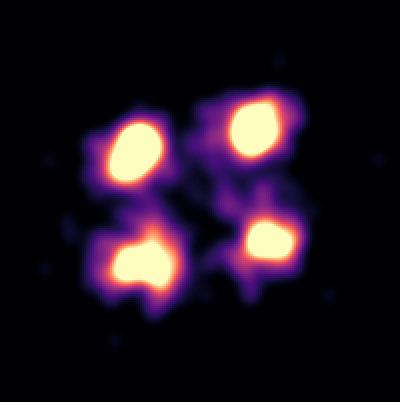
\includegraphics[width=\plotwidth]{figures/data/exp_counting/4bs_origami_1.png}
    \&
    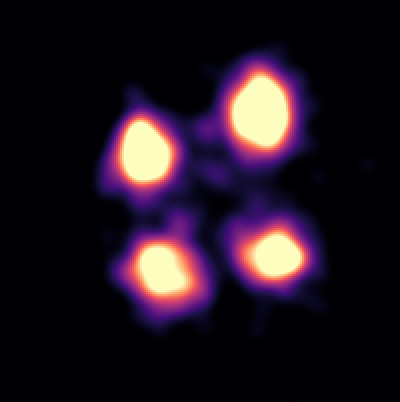
\includegraphics[width=\plotwidth]{figures/data/exp_counting/4bs_origami_2.png}
    \&
    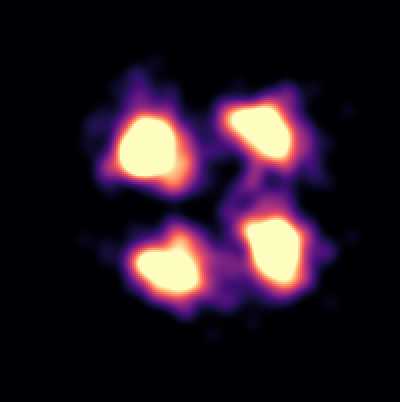
\includegraphics[width=\plotwidth]{figures/data/exp_counting/4bs_origami_3.png}
    \&
    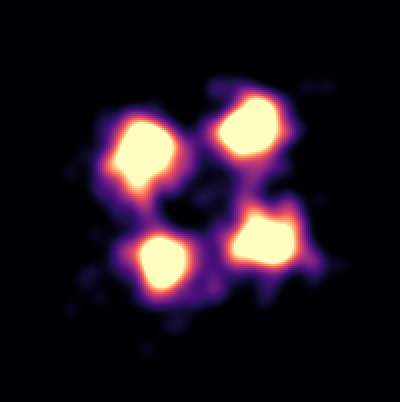
\includegraphics[width=\plotwidth]{figures/data/exp_counting/4bs_origami_4.png}
    \\
  };

  % scale bar
  \node[
    rectangle,
    minimum width=0.25\plotwidth, % images are 400px, 1/4 is 100px and that is 20nm
    fill=white,
    anchor=south east,
    inner sep=0pt,
    outer sep=2mm] (scalebar) at (samples-1-4.south east) {};
  \node[anchor=south,white] at (scalebar.center) {\tiny $20 \micrometer$};
\end{tikzpicture}
%
  \end{panel}
  \begin{panel}{(d)}{0.2\textwidth}
    \hspace{2mm}%
    \def\plotwidth{0.8\textwidth}%
    \def\plotheight{20mm}%
    \tikzsetnextfilename{exp_mean_probabilities_n1}%
\begin{tikzpicture}

  \pgfplotsset{every axis/.style={name=n1}}
  \def\posteriorcsv{figures/data/exp_counting/mean_probabilities.csv}
  \def\posteriorcol{n1_prob}
  \input{figures/plots/p_n_given_x.plot}
  \node[anchor=south] at (n1.outer north) {origami with $\n=1$};

\end{tikzpicture}
%
  \end{panel}
  \begin{panel}{(e)}{0.2\textwidth}
    \hspace{2mm}%
    \def\plotwidth{0.8\textwidth}%
    \def\plotheight{20mm}%
    \tikzsetnextfilename{exp_mean_probabilities_n4}%
\begin{tikzpicture}

  \pgfplotsset{every axis/.style={name=n4}}
  \def\posteriorcsv{figures/data/exp_counting/mean_probabilities.csv}
  \def\posteriorcol{n4_prob}
  \input{figures/plots/p_n_given_x.plot}
  \node[anchor=south] at (n4.outer north) {origami with $\n=4$};

\end{tikzpicture}
%
  \end{panel}

  \caption{
    \panelref{a, b} Experimental traces with super-resolution confirmed counts of one (a) and four (b), and \ours fits
    %
    \panelref{c} Super-resolution visualization of origamis made with four binding sites.
    %
    \panelref{d, e} Average \ours posterior distributions of 112 traces with a known $n$ of one (d) and 
    110 traces with a known $n$ of four (e)
  }
  \label{fig:results:experimental}
\end{figure*}


\subsection{Simulated Experiments}
% Simulated traces based on experimentally relevant parameters
Running \ours as a forward model, traces were generated for counts N=1 to 30
	(\figref{fig:results:sim_counting}a,b), with experimentally relevant parameters. 
	%
	Camera parameters were determined from an empirical calibration of the
	sCMOS camera (\parametersc: \camgain=2.17, \camoffset=4791, \camvar=774), 
	and kinetic (\parameterst: \pon=0.036, \poff=0.028), and emission parameters (\parameterse: \re=2.79, \rb=6.77) were determined through an
	initial experiment, and closely match those reported in literature \cite{stein_2021}.
	%
	Traces were generated for 4000 frames, corresponding to an imaging time of 14 minutes.

% priors were placed on camera parameters, but all others were uniform
While fitting, tight gaussian priors were placed on the camera parameters because these were empirically determined.
	%
	Flat uniform priors were place on the kinetic parameters, allowing the model to fit blinking rates without external bias.
	%
	Loose priors were placed on the emission parameters (\rb, \re) to prevent overcounting (discussed further in discussion). 
	% how we got these priors
	The prior on \rb can be experimentally determined by averaging the intensity of pixels immediately outside the spot ROI.
	The prior on \re was determined by first fitting a count of \n=1 to the trace.
	%
	Given the definitions of \pon and \poff, the most common transition from state $z$ will be to state $\z{} \pm 1$, a switch of a single emitter.
	It follows that the distribution of all observed $z$-states will be unimodal, and that whichever \z{}-state is the most common, 
	the second most common will be $\z{} \pm 1$. Therefore fitting $n=1$ will capture this transition 
	and as a result accurately estimate \re (the photon emission rate of a single emitter).
	%
	

% blinx can count!
\ours successfully fit simulated traces with counts up to N=30 (\figref{fig:results:sim_counting}c).
	%
	For N=10 and below, \ours fit the correct count, with a significantly higher likelihood than all other possibilities. 
	%
	Above N=10 the likelihood of other possible counts increased, but the posterior distribution remained centered on the correct count.
	%
	Importantly, \ours is able to fit the correct count,
	despite the fact that not every state is visited \ie the model is not just counting the number of peaks in the intensity histogram (\figref{fig:results:sim_counting}a,b).
	% blinx outperforms lbFCS, counting up to 30 
	This is a tripling in performance compared to lbFCS, which counted accurately up to N=7, but failed to estimate higher counts.
	% main limitation of lbFCS is estimation of the "step size" corresponding to r_e
	Upon further analysis, the main limitation of lbFCS is the estimation of the intensity of a single emitter, corresponding to $r_e$ in \ours. 
	%
	lbFCS relies on a histogram based method to determine this value, while \ours is able to jointly optimize this parameter with the others.
	%
	%If this value is first estimated by \ours, then supplied to lbFCS, performance is significantly rescued (SI Figure).

% Longer traces lead to better fits
Next, the effect of trace length on counting accuracy (\figref{fig:results:sim_counting}d) was investigated.
	%
	As expected accuracy increased and variance of the posterior distribution decreased, 
	as the number of observations increased.
	% Also notice a underestimation of count with low trace length
	Interestingly, for short trace lengths, \ours underestimated the true count. 
	%
	Underestimating more severely as the true count increased.
	% This is most likely due to the system only occupying a subset of all possible zs in this short time
	This is likely because only a subset of possible states were observed in this short time.

% there is a lower bound to SNR, below a specific SNR, model maximally overcounts
To investigate the effect of noise on counting ability, the variance of the readout noise \camvar was tuned to produce a 
	series of traces with differing SNR values. 
	%
	Because noise in our model is proportional to intensity, quantifying the SNR of a trace 
	is not trivial. 
	%
	For simplicity, here we define SNR as the difference in intensity between 
	the first two states (\z{0} and \z{1}) divided by the square root of the sum of the variances of both states. 
	%
	In effect this is the upper bound of SNR for a given trace. 
	%
	The base model, with experimentally measured \camvar corresponds to an SNR of 9. 
	%
	\ours shows similar performance down to an SNR as low as 4 (\figref{fig:results:sim_counting}e). 
	%
	Interestingly, at SNR's below 4, \ours estimates the count as 25, the highest \n tested, no matter the true count. 
	%
	This is due to the low probability of observing states far from the mean of our intensity model, and is further expanded on in the discussion. 


\subsection{Kinetic sweep}
	% blinx lets us look at effects of changing experimental conditions
To determine the effect of blinking kinetics on the counting ability of \ours, traces were simulated with a range of kinetic parameters, 
	while holding all other parameters constant.
	%
	Using the poisson distribution to convert from $k_{on}$ and $k_{off}$ to \pon and \poff,
	it was ensured that this range covered experimentally relevant kinetics from literature,
	qPAINT: (\pon, \poff) = (0.006, 0.2) \cite{jungmann_2016} and lbFCS (0.02, 0.02) \cite{stein_2021}. 
	%
	Traces with true counts from 1 to 20 were simulated and fit.
	%
	The resulting posterior for all $n$s 1 to 20, was then reduced to the weighted mean square error from a perfect fit for comparison (\figref{fig:results:campare_kinetics}a).
	%
	
\ours preforms well in regimes of high \pon and low \poff, and sees a significant decrease in performance as \poff increases. 
	%
	In the extreme of the qPAINT regime, \ours is unable to count, estimating a \n = 1 or 2 regardless of the true value.
	%
	The clear difference between these two regimes can be visualized through representative traces, and intensity histograms (\figref{fig:results:campare_kinetics}c,d),
	both of which have a true count of \n=10.
	%
	In the low \pon / high \poff regime, a majority of time is spent only in the lowest two states and without 
	any prior knowledge the count of these trace becomes indistinguishable.
	% do a better job connecting few states observed --> indistinguishable 
	% 
	In contrast, in the high \pon / low \poff regime a majority of the states are visited, and \ours 
	is able to accurately recover the correct count.

% Experimental
% Do we need to explain how DNA-PAINT works
In DNA-PAINT, the blinking rate is determined by the kinetics of single-stranded DNA binding,
which in turn are dependant on experimental conditions such as temperature and concentration, and sequence.
	%
	As a result, the kinetic parameters \pon and \poff of our model, are can be 
	tuned by adjusting the temperature and imager concentration.
	%
	Imaging DNA-origami with a known count of $\n=1$ at 25 C and an 
	imager concentration of 10 nM, we measured $\pon=0.028$ and $\poff=0.072$ 
	(\figref{fig:results:campare_kinetics}b).
	%
	Which places these conditions firmly in the poor counting 
	accuracy regime of $\pon < \poff$ (\figref{fig:results:campare_kinetics}a). % fix
	
In order to move to a more favorable kinetic regime, 
we increased the imager concentration and decreased the temperature.
	%
	Increasing imger concentration to 30 nM raised \pon to 0.071 and 
	decreasing temperature to 13 C decreased \poff to 0.037 
	(\figref{fig:results:campare_kinetics}b).
	%
	The effects of temperature and concentration were largely independent 
	of one another providing precise control over the kinetic parameters. % cite jungmann paper
	%
	We also observed a significant decrease in SNR with decreasing temperature, 
	and with increasing concentration. 
	%
	This was an expected side effect of increasing concentration, as more imager would increase \rb.
	%
	But the effect of temperature on SNR was surprising. 
	We hypothesize that this is due to the stabilization partial 
	binding between imager and docker strands at low temperatures.
	%
	Accounting for both the increase in counting accuracy and the decrease 
	in SNR, imaging conditions of 20 nM and 13 C were chosen as optimal.

\subsection{qPAINT Kinetic Regime}
% qPAINT operates in a different kinetic regime that lbFCS
qPAINT is based on an accurate measure of the average dark time between blinking events. 
	%
	As a result, this method operates in an entirely different kinetic regime than lbFCS, where blinking 
	events are short and infrequent (\figref{fig:results:qpaint_counting}a,b).
	% this presents challenges to blinx
	This regime presents a challenge to \ours. 
	%
	If the only states ever observed are z=0 or 1 (off or on), there is not enough information in the system to estimate count without prior knowledge.
	% qPAINT relies on a calibration of kinetics
	qPAINT, faces the same limitation, and relies on a calibration of the blinking kinetics of a single binding site.
	% However, blinx is fully Bayesian and we can overcome these challenges by tightening priors
	\ours, as a fully Bayesian model can easily incorporate the same calibration as priors of the kinetic parameters
	and once again accurately count up to N=30 (\figref{fig:results:qpaint_counting}c).

% qPAINT undercounts but blinx does not
Due to the stochastic nature of blinking, multiple binding sites can blink at the same time, which becomes increasingly likely at higher counts.
	%
	This is not compatible with the qPAINT assumption of well separated, single binding-site blinking events, 
	and as a result, qPAINT begins to underestimate molecular count, (especially noticeable above N=20, (\figref{fig:results:qpaint_counting}c)). 
	% blinx avoids this problem
	The blinking of multiple binding sites at the same time point, 
	is compatible and accounted for in the transition model of blinx 
	and as a result, blinx accurately estimates the count even at higher N.
	

\subsection{Experimental Counting}
% briefly describe experimental setup
To experimentally validate the counting performance of \ours, DNA-Origami, which allows fine control over the number of emitters, was used.
	% Why DNA origami
	DNA-Origamis were designed containing 1 and 4 DNA-PAINT docker strands, spaced in a grid 20 \nanometer apart. 
	%
	This distance was specifically chosen, so that the true number of docker strands could be visually confirmed through super-resolution post-processing.
	%
	Incorporation efficiency is roughly 80 percent for each docker site \cite{strauss_2018}, so only a fraction of the origamis were expected to contain all 4 dockers. 
	% 
	Origamis were first imaged at 13 C, low laser power, and 20 nM imager concentration to collect traces for counting with \ours (\figref{fig:results:experimental}a,b).
	%
	Then the system was allowed to warm to 25C, a buffer exchange performed and new imager added at 10 nM, and the origamis were imaged again at high laser power,
	and post-processed to obtain super-resolution ground truth (\figref{fig:results:experimental}c).
	%
	Only origamis that had a visual count matching the designed count (1 or 4) were selected for analysis with \ours.

Of 131 traces with a known count of 1, \ours correctly counted 112 (85\%) and the maximum estimated count was 3 (1/131) (\figref{fig:results:experimental}e).
	%
	For the traces with a known count of 4, 71/110 (65\%) were correctly identified as 4, and 103/110 were identified as between 3 and 5.
	%
	% A more detailed analysis of wrongly counted traces is found in the SI.
	%
	Importantly, no filtering or preprocessing was done on the measured traces, and many of the incorrect counts were due to low trace SNR. % quantify this??

\section{Conclusions}

One advantage of \ours is that intensity parameters and blinking rates are jointly estimated, improving the fit of all parameters compared to \lbfcs, and resulting in a doubling of the counting ability. 
%
Another advantage is that \ours calculates a likelihood, thus making different models and counts directly comparable. 
%

\ours is built on a few assumptions, most important being that all emitters behave independently. While this assumption holds true for idealized scenarios, emitters can have effects on both the intensity and rate parameters of their immediate neighbors.
%
Another assumption is that all emitters in a spot blink at the same rate and that their parameters are constant over time. However, blinking rates and intensity are dependent on the local nano environment, and small variations in this environment could lead to large differences between emitters.
%
Moreover, these parameters are also highly dependent on experimental conditions, \ie, temperature, which can fluctuate over time without proper controls.
%
Nevertheless, we did not find those potential limitations to be detrimental in
preliminary SMLM imaging experiments.
%
In conclusion, we believe that holistic methods like \ours are key for future
experiment designs that require counting large numbers of fluorescent emitters.

\bibliography{references}
\bibliographystyle{icml2023}

\end{document}
